% Two-column system overview, queued early so it lands before the method text.
\begin{figure*}[!t]
\centering
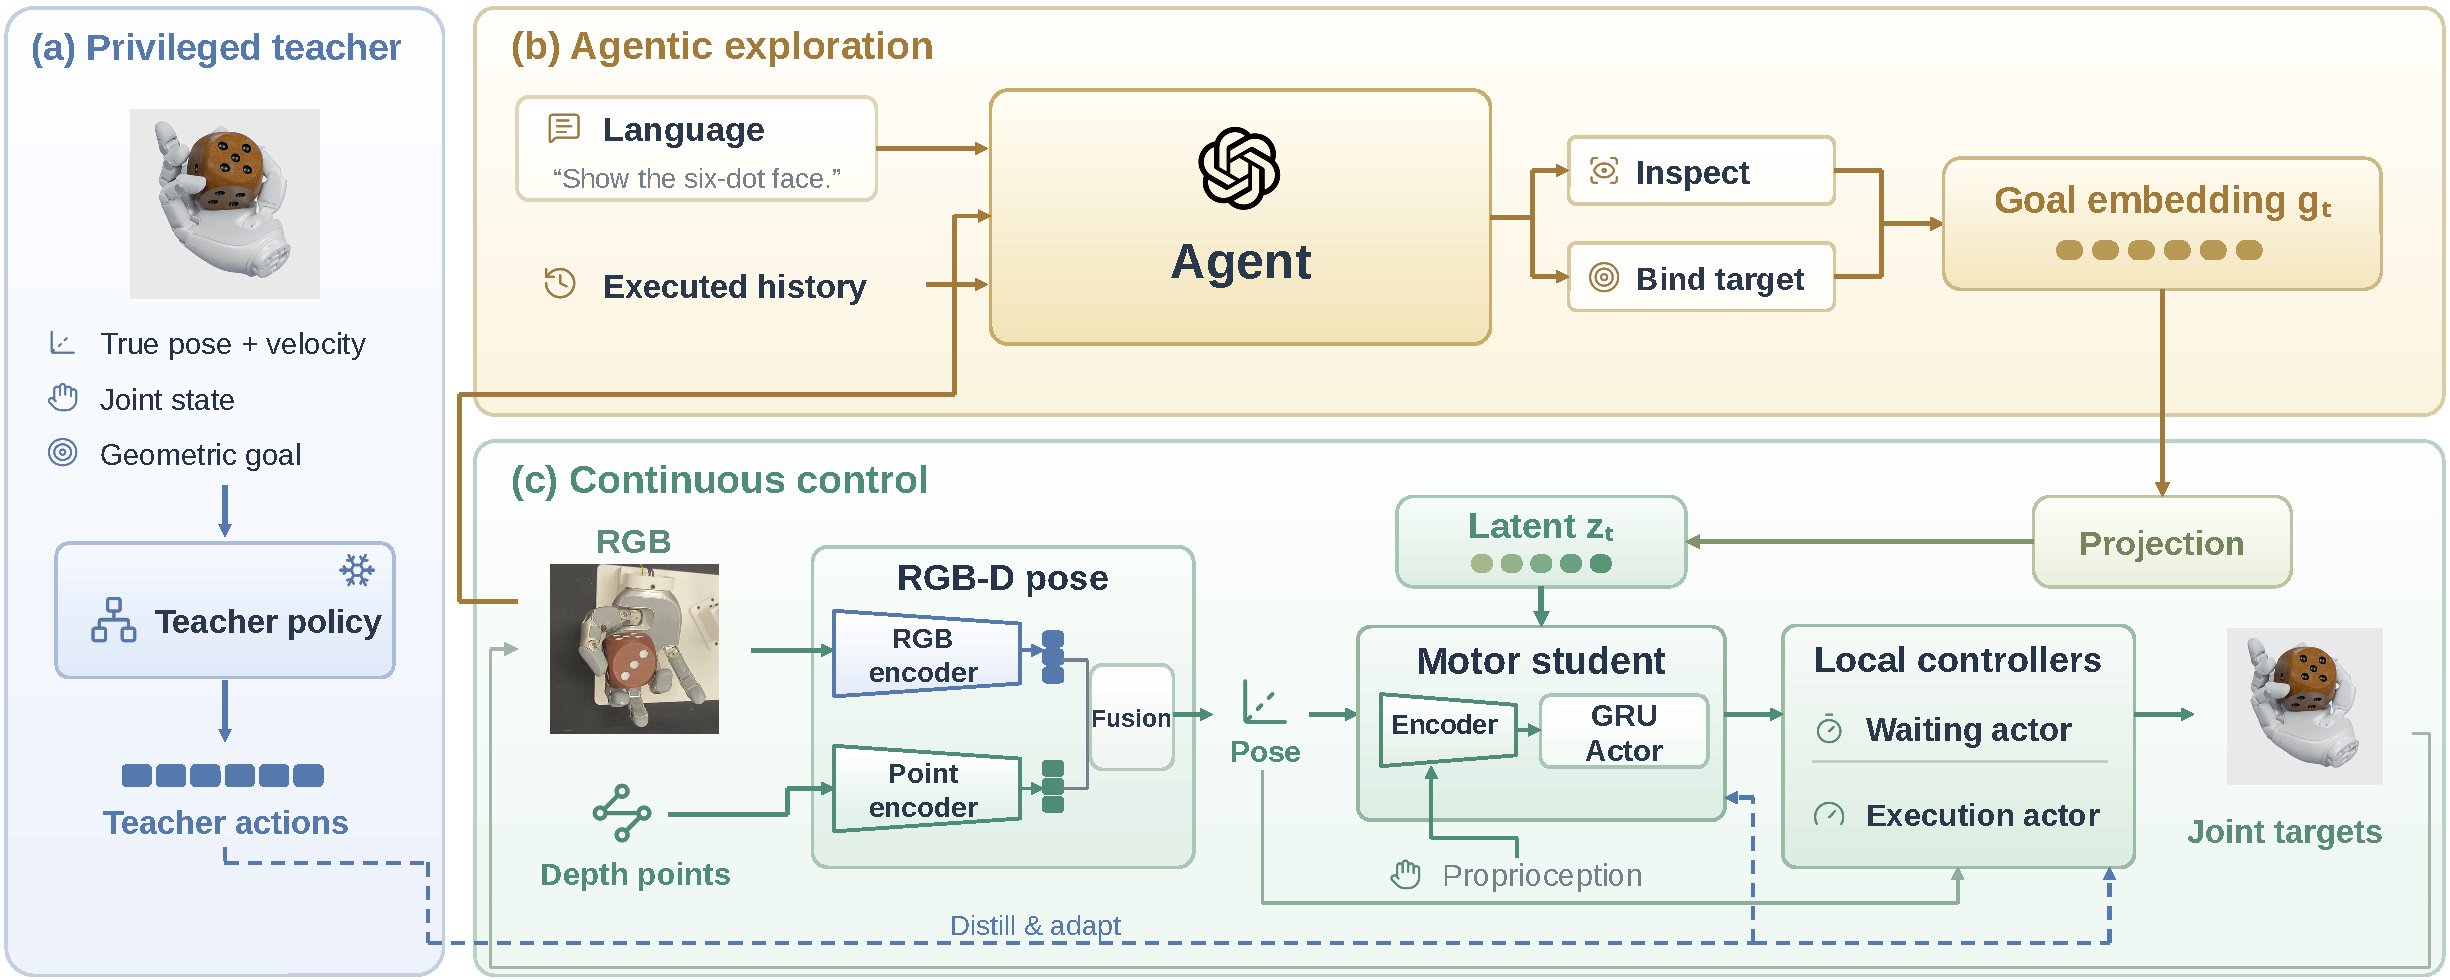
\includegraphics[width=0.96\textwidth]{figures/imported/v11/reveal_pipeline_v11.pdf}
\caption{\textbf{REVEAL training and deployment.} (a) A privileged teacher with full simulator state is trained for the Revo3 hand. (b) At deployment the agent reads the instruction, the current view and the history of executed actions, and returns either an inspection or a target binding; its output is a goal embedding $g_t$ drawn from the skill bank. (c) Underneath, an RGB-D pose estimator fuses image features with measured surface points, a motor student turns pose and goal into joint targets, and waiting and execution controllers adjust those targets while the agent is still reasoning. The teacher is used only for supervision and the state decoder only in training.}
\label{fig:pipeline}
\end{figure*}
